\hypertarget{ux4f7fux7528-web-ux6846ux67b6}{%
\subsection{使用 Web 框架}\label{ux4f7fux7528-web-ux6846ux67b6}}

了解了 WSGI 框架,我们发现:其实一个 Web App,就是写一个 WSGI
的处理函数,针对每个 HTTP 请求进行响应。

但是如何处理 HTTP 请求不是问题,问题是如何处理 100 个不同的 URL。

每一个 URL 可以对应 GET 和 POST 请求,当然还有 PUT、DELETE
等请求,但是我们通常只考虑最常见的 GET 和 POST 请求。

一个最简单的想法是从\texttt{environ}变量里取出 HTTP
请求的信息,然后逐个判断:

\begin{pythoncode}
def application(environ, start_response):
    method = environ['REQUEST_METHOD']
    path = environ['PATH_INFO']
    if method=='GET' and path=='/':
        return handle_home(environ, start_response)
    if method=='POST' and path='/signin':
        return handle_signin(environ, start_response)
    ...
\end{pythoncode}

只是这么写下去代码是肯定没法维护了。

代码这么写没法维护的原因是因为 WSGI 提供的接口虽然比 HTTP
接口高级了不少,但和 Web App 的处理逻辑比,还是比较低级,我们需要在 WSGI
接口之上能进一步抽象,让我们专注于用一个函数处理一个 URL,至于 URL
到函数的映射,就交给 Web 框架来做。

由于用 Python 开发一个 Web 框架十分容易,所以 Python 有上百个开源的 Web
框架。这里我们先不讨论各种 Web 框架的优缺点,直接选择一个比较流行的 Web
框架------\href{http://flask.pocoo.org/}{Flask} 来使用。

用 Flask 编写 Web App 比 WSGI 接口简单(这不是废话么,要是比 WSGI
还复杂,用框架干嘛?),我们先用\texttt{pip}安装 Flask:

\begin{pythoncode}
$ pip install flask
\end{pythoncode}

然后写一个\texttt{app.py},处理 3 个 URL,分别是:

\begin{itemize}
\item
  \texttt{GET\ /}:首页,返回\texttt{Home};
\item
  \texttt{GET\ /signin}:登录页,显示登录表单;
\item
  \texttt{POST\ /signin}:处理登录表单,显示登录结果。
\end{itemize}

注意噢,同一个 URL\texttt{/signin}分别有 GET 和 POST
两种请求,映射到两个处理函数中。

Flask 通过 Python
的\href{https://www.liaoxuefeng.com/wiki/1016959663602400/1017451662295584}{装饰器}在内部自动地把
URL 和函数给关联起来,所以,我们写出来的代码就像这样:

\begin{pythoncode}
from flask import Flask
from flask import request

app = Flask(__name__)

@app.route('/', methods=['GET', 'POST'])
def home():
    return '<h1>Home</h1>'

@app.route('/signin', methods=['GET'])
def signin_form():
    return '''<form action="/signin" method="post">
              <p><input ></p>
              <p><input ></p>
              <p><button type="submit">Sign In</button></p>
              </form>'''

@app.route('/signin', methods=['POST'])
def signin():
    # 需要从request对象读取表单内容:
    if request.form['username']=='admin' and request.form['password']=='password':
        return '<h3>Hello, admin!</h3>'
    return '<h3>Bad username or password.</h3>'

if __name__ == '__main__':
    app.run()
\end{pythoncode}

运行\texttt{python\ app.py},Flask 自带的 Server
在端口\texttt{5000}上监听:

\begin{pythoncode}
$ python app.py 
 * Running on http://127.0.0.1:5000/
\end{pythoncode}

打开浏览器,输入首页地址\texttt{http://localhost:5000/}:

 
 \begin{figure}[htp]
	\centering
	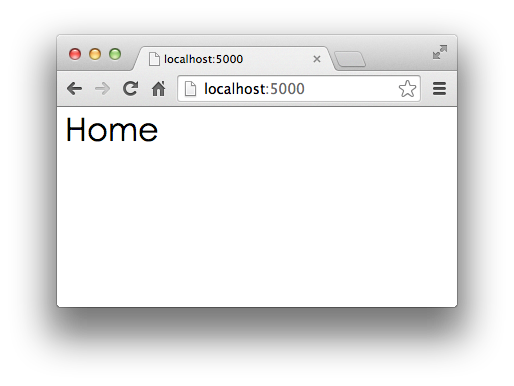
\includegraphics[width=0.6\linewidth]{fig/951373547960800.png}
\end{figure}


首页显示正确!

再在浏览器地址栏输入\texttt{http://localhost:5000/signin},会显示登录表单:

 
 \begin{figure}[htp]
	\centering
	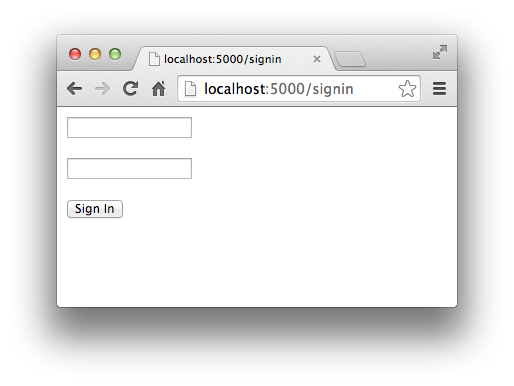
\includegraphics[width=0.6\linewidth]{fig/951373657012736.png}
\end{figure}


输入预设的用户名\texttt{admin}和口令\texttt{password},登录成功:

 
 \begin{figure}[htp]
	\centering
	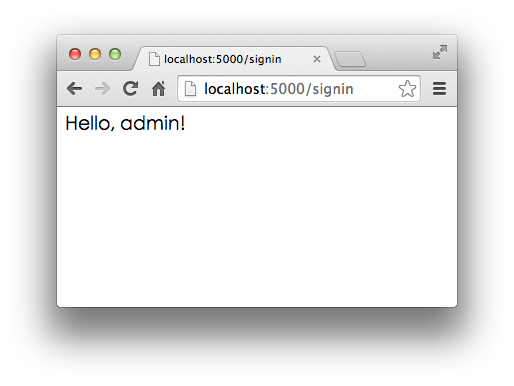
\includegraphics[width=0.6\linewidth]{fig/951373763967808.png}
\end{figure}


输入其他错误的用户名和口令,登录失败:

 
 \begin{figure}[htp]
	\centering
	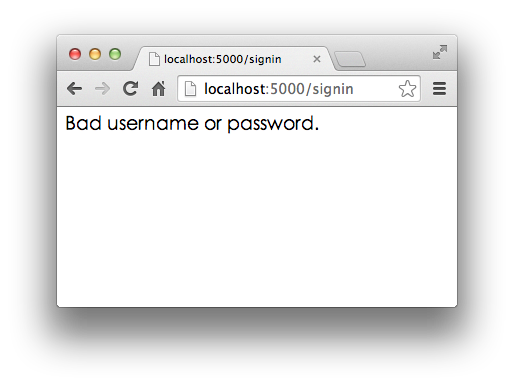
\includegraphics[width=0.6\linewidth]{fig/951373786253056.png}
\end{figure}


实际的 Web App
应该拿到用户名和口令后,去数据库查询再比对,来判断用户是否能登录成功。

除了 Flask,常见的 Python Web 框架还有:

\begin{itemize}
\item
  \href{https://www.djangoproject.com/}{Django}:全能型 Web 框架;
\item
  \href{http://webpy.org/}{web.py}:一个小巧的 Web 框架;
\item
  \href{http://bottlepy.org/}{Bottle}:和 Flask 类似的 Web 框架;
\item
  \href{http://www.tornadoweb.org/}{Tornado}:Facebook 的开源异步 Web
  框架。
\end{itemize}

当然了,因为开发 Python 的 Web 框架也不是什么难事,我们后面也会讲到开发
Web 框架的内容。

\hypertarget{ux5c0fux7ed3}{%
\subsubsection{小结}\label{ux5c0fux7ed3}}

有了 Web 框架,我们在编写 Web 应用时,注意力就从 WSGI 处理函数转移到 URL
+ 对应的处理函数,这样,编写 Web App 就更加简单了。

在编写 URL 处理函数时,除了配置 URL 外,从 HTTP
请求拿到用户数据也是非常重要的。Web 框架都提供了自己的 API
来实现这些功能。Flask
通过\texttt{request.form{[}\textquotesingle{}name\textquotesingle{}{]}}来获取表单的内容。

\hypertarget{ux53c2ux8003ux6e90ux7801}{%
\subsubsection{参考源码}\label{ux53c2ux8003ux6e90ux7801}}

\href{https://github.com/michaelliao/learn-python3/blob/master/samples/web/do_flask.py}{do\_flask.py}

